\documentclass[report.tex]{subfiles}		
\begin{document}
\section{Encryption process} \label{sec:encryption process}
Encrypting data with the AES algorithm begins by copying the input data to a state block and then adding the first round key. The state block is then transformed in $N_r-1$ rounds, where each round consists of four transformations:
\begin{enumerate}
\item Substitution using a substitution table
\item Row shifting
\item Column mixing
\item Round key addition
\end{enumerate}
In the final round, no column mixing is performed since it does not add to the security of the encryption.

As the last step, the state block is copied to the output block.

\clearpage

\begin{figure}[h]
\centering
\begin{tikzpicture}[node distance = 30pt, auto]
    % Place nodes
    \node [cloud] (input) {Input data};
    \node [state,     below of=input]                      (state)  {State block};
    \node [roundkey,  below of=state, node distance=40pt]  (init)   {Add round key};
    \node [subbyte,   below of=init,  node distance=50pt]  (sbox)   {1 - SubBytes};
    \node [shiftrow,  below of=sbox]                       (shift)  {2 - Shift rows};
    \node [mixcolumn, below of=shift]                      (mix)    {3 - Mix columns};
    \node [roundkey,  below of=mix]                        (round)  {4 - Add round key};
    \node [subbyte,   below of=round, node distance=50pt]  (sbox2)  {SubBytes};
    \node [shiftrow,  below of=sbox2]                      (shift2) {Shift rows};
    \node [roundkey,  below of=shift2]                     (round2) {Add round key};
	\node [cloud,     below of=round2, node distance=40pt] (output) {Output data};
    % Draw interconnecting lines
    \path [line,dashed] (input)  -- (state);
    \path [line]        (state)  -- (init);
    \path [line]        (init)   -- (sbox);
    \path [line]        (sbox)   -- (shift);
    \path [line]        (shift)  -- (mix);
    \path [line]        (mix)    -- (round);
    \path [line]        (round)  -- (sbox2);
    \path [line]        (sbox2)  -- (shift2);
    \path [line]        (shift2) -- (round2);
    \path [line,dashed] (round2) -- (output);
    % Draw "repeat" line
    \path [line, rounded corners=10pt] ($ (round.south)!0.3!(sbox2.north) $) -- 
               ++(80pt,0) --
                 ($ (init.south)!0.70!(sbox.north) + (80pt,0) $) ->
                 ($ (init.south)!0.70!(sbox.north) $);
    % Draw dashed separators (these actually does the centering for us)
    \draw [dashed] ($ (input.south)!0.5!(state.north)+(-\linewidth*0.25,0) $) --
                   ($ (input.south)!0.5!(state.north)+(\linewidth*0.75,0) $);
    \draw [dashed] ($ (init.south)!0.5!(sbox.north)+(-\linewidth*0.25,0) $) --
                   ($ (init.south)!0.5!(sbox.north)+(\linewidth*0.75,0) $);
    \draw [dashed] ($ (round.south)!0.5!(sbox2.north)+(-\linewidth*0.25,0) $) --
                   ($ (round.south)!0.5!(sbox2.north)+(\linewidth*0.75,0) $);
    \draw [dashed] ($ (round2.south)!0.5!(output.north)+(-\linewidth*0.25,0) $) --
                   ($ (round2.south)!0.5!(output.north)+(\linewidth*0.75,0) $);

    % Place right hand text
    \path ($ (input)+(\linewidth*0.5,0) $) node[align=center,text width=80pt]
	    {\huge Input};
    \path ($ (state.south)!0.5!(init.north)+(\linewidth*0.5,0) $) node[align=center,text width=80pt]
	    {\huge Initial round};
	\path ($ (shift.south)!0.5!(mix.north)+(\linewidth*0.5,0) $) node[align=center,text width=80pt]
	    {\huge $N_r-1$ main rounds};
	\path ($ (shift2)+(\linewidth*0.5,0) $) node[align=center,text width=80pt]
	    {\huge Final round};
	\path ($ (output)+(\linewidth*0.5,0) $) node[align=center,text width=80pt]
	    {\huge Output};
\end{tikzpicture}
\caption{Encryption process overview}
\end{figure}

\clearpage

\subsection{Substitution using a substitution table}\label{sec:substitution}
Each byte in a state block is represented by two hexadecimal digits. These two digits are then used as row and column index in the substitution table in figure \ref{fig:s-box}. E.g. the value $\textrm{42}_{10}$ is $\textrm{2A}_{16}$ in hexadecimal form and would be transformed to $\textrm{E5}_{16}$.

\begin{figure}[h]
\centering
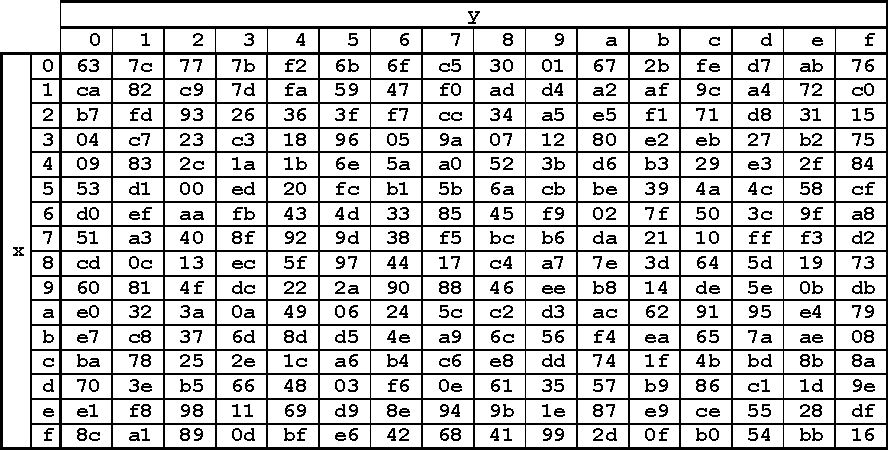
\includegraphics[width=\linewidth]{s-box}
\caption{Substitution table. Source: fips}
\label{fig:s-box}
\end{figure}

This transformation is performed on every byte in a state block.

\subsection{Row shifting}
Row shifting means that each row in a state block is cyclically shifted left $N$ times, where $N$ is the row number - 1, i.e. the first row is shifted $0$ times, the second row $1$ time, etc.

\begin{figure}[h]
\centering
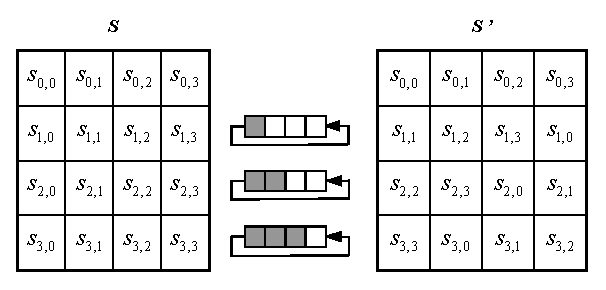
\includegraphics[width=\linewidth]{row_shifting}
\caption{Illustration of row shifting. Source: fips}
\label{fig:row_shifting}
\end{figure}

\subsection{Column mixing}
The mix column transformation is done by multiplying each column by a given matrix as shown in equation \ref{eq:mix columns} below.
\begin{equation}\label{eq:mix columns}
	\begin{bmatrix}
	S_{0,c}^\text{'} \\
	S_{1,c}^\text{'} \\
	S_{2,c}^\text{'} \\
	S_{3,c}^\text{'}
	\end{bmatrix}
	=
	\begin{bmatrix}
	02 & 03 & 01 & 01 \\
	01 & 02 & 03 & 01 \\
	01 & 01 & 02 & 03 \\
	03 & 01 & 01 & 02
	\end{bmatrix}
	\bullet
	\begin{bmatrix}
	S_{0,c} \\
	S_{1,c} \\
	S_{2,c} \\
	S_{3,c}
	\end{bmatrix}
	\text{for }0 \leq c \leq 3
\end{equation}

\subsection{Round key addition}
The last step of every round is to add the round key to the state block.
\begin{equation}\label{eq:round key}
	\mathbf{S^\text{'}} = 
	\overbrace{
	\begin{bmatrix}
	S_{0,0} & S_{0,1} & S_{0,2} & S_{0,3} \\
	S_{1,0} & S_{1,1} & S_{1,2} & S_{1,3} \\
	S_{2,0} & S_{2,1} & S_{2,2} & S_{2,3} \\
	S_{3,0} & S_{3,1} & S_{3,2} & S_{3,3}
	\end{bmatrix}}^\text{State block}
	\bigoplus
	\overbrace{
	\begin{bmatrix}
	W_{0,0} & W_{0,1} & W_{0,2} & W_{0,3} \\
	W_{1,0} & W_{1,1} & W_{1,2} & W_{1,3} \\
	W_{2,0} & W_{2,1} & W_{2,2} & W_{2,3} \\
	W_{3,0} & W_{3,1} & W_{3,2} & W_{3,3}
	\end{bmatrix}}^\text{Round key}
\end{equation}
\end{document}